% Created by tikzDevice version 0.6.2 on 2012-04-20 14:43:10
% !TEX encoding = UTF-8 Unicode
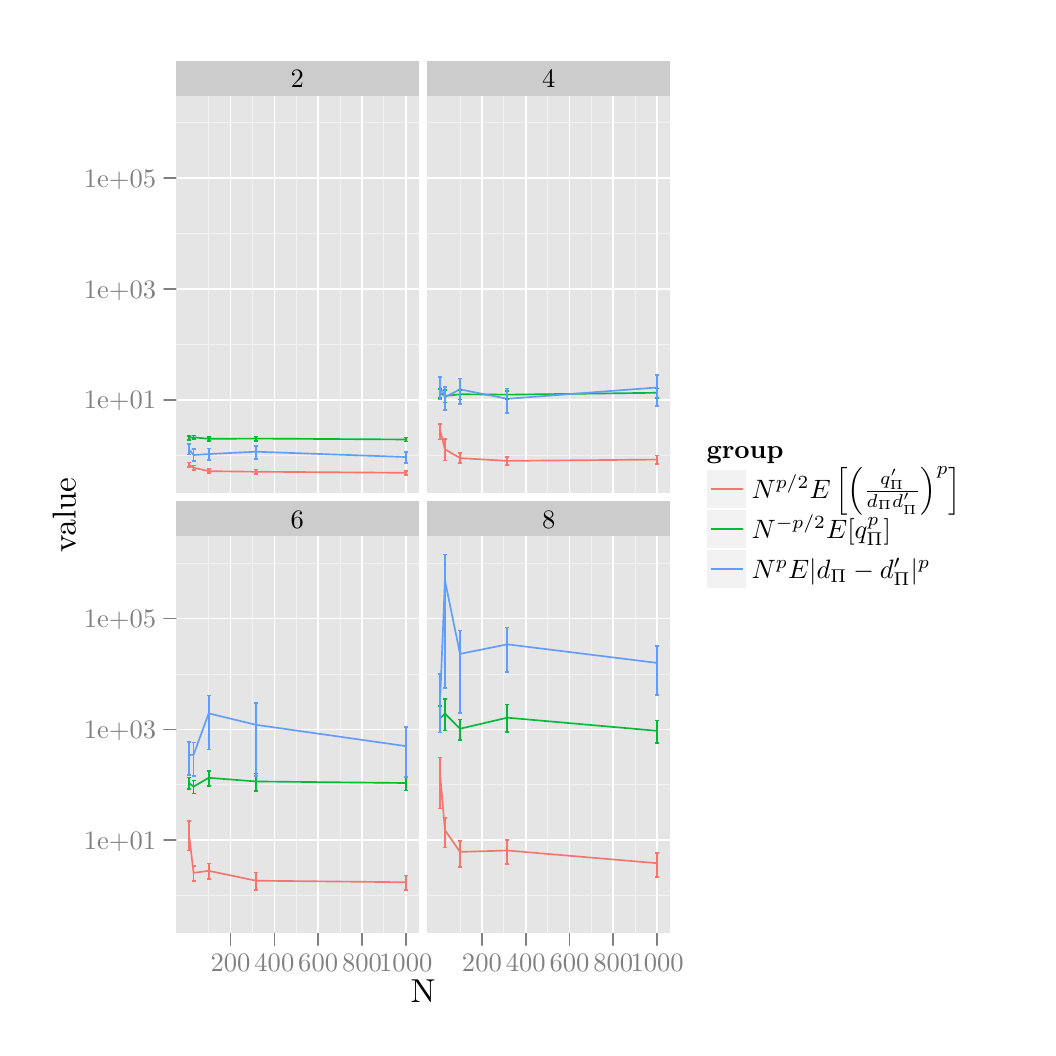
\begin{tikzpicture}[x=1pt,y=1pt]
\definecolor[named]{drawColor}{rgb}{0.00,0.00,0.00}
\definecolor[named]{fillColor}{rgb}{1.00,1.00,1.00}
\fill[color=fillColor,fill opacity=0.00,] (0,0) rectangle (361.35,361.35);
\begin{scope}
\path[clip] (  0.00,  0.00) rectangle (361.35,361.35);
\definecolor[named]{drawColor}{rgb}{0.41,0.16,0.58}
\end{scope}
\begin{scope}
\path[clip] (  0.00,  0.00) rectangle (361.35,361.35);
\definecolor[named]{drawColor}{rgb}{0.41,0.16,0.58}
\end{scope}
\begin{scope}
\path[clip] (  0.00,  0.00) rectangle (361.35,361.35);
\definecolor[named]{drawColor}{rgb}{0.41,0.16,0.58}
\end{scope}
\begin{scope}
\path[clip] (  0.00,  0.00) rectangle (361.35,361.35);
\definecolor[named]{drawColor}{rgb}{0.41,0.16,0.58}
\end{scope}
\begin{scope}
\path[clip] (  0.00,  0.00) rectangle (361.35,361.35);
\definecolor[named]{drawColor}{rgb}{0.41,0.16,0.58}
\end{scope}
\begin{scope}
\path[clip] (  0.00,  0.00) rectangle (361.35,361.35);
\definecolor[named]{drawColor}{rgb}{0.41,0.16,0.58}
\end{scope}
\begin{scope}
\path[clip] (  0.00,  0.00) rectangle (361.35,361.35);
\definecolor[named]{drawColor}{rgb}{0.41,0.16,0.58}
\end{scope}
\begin{scope}
\path[clip] (  0.00,  0.00) rectangle (361.35,361.35);
\definecolor[named]{drawColor}{rgb}{0.41,0.16,0.58}
\end{scope}
\begin{scope}
\path[clip] ( 53.55,193.18) rectangle (141.36,336.67);
\definecolor[named]{drawColor}{rgb}{0.41,0.16,0.58}
\end{scope}
\begin{scope}
\path[clip] (  0.00,  0.00) rectangle (361.35,361.35);
\definecolor[named]{drawColor}{rgb}{0.41,0.16,0.58}
\end{scope}
\begin{scope}
\path[clip] (144.37,193.18) rectangle (232.17,336.67);
\definecolor[named]{drawColor}{rgb}{0.41,0.16,0.58}
\end{scope}
\begin{scope}
\path[clip] (  0.00,  0.00) rectangle (361.35,361.35);
\definecolor[named]{drawColor}{rgb}{0.41,0.16,0.58}
\end{scope}
\begin{scope}
\path[clip] ( 53.55, 34.03) rectangle (141.36,177.53);
\definecolor[named]{drawColor}{rgb}{0.41,0.16,0.58}
\end{scope}
\begin{scope}
\path[clip] (  0.00,  0.00) rectangle (361.35,361.35);
\definecolor[named]{drawColor}{rgb}{0.41,0.16,0.58}
\end{scope}
\begin{scope}
\path[clip] (144.37, 34.03) rectangle (232.17,177.53);
\definecolor[named]{drawColor}{rgb}{0.41,0.16,0.58}
\end{scope}
\begin{scope}
\path[clip] (  0.00,  0.00) rectangle (361.35,361.35);
\definecolor[named]{drawColor}{rgb}{0.41,0.16,0.58}
\end{scope}
\begin{scope}
\path[clip] (  0.00,  0.00) rectangle (361.35,361.35);
\definecolor[named]{drawColor}{rgb}{0.41,0.16,0.58}
\end{scope}
\begin{scope}
\path[clip] (  0.00,  0.00) rectangle (361.35,361.35);
\definecolor[named]{drawColor}{rgb}{0.41,0.16,0.58}
\end{scope}
\begin{scope}
\path[clip] (  0.00,  0.00) rectangle (361.35,361.35);
\definecolor[named]{drawColor}{rgb}{0.41,0.16,0.58}
\end{scope}
\begin{scope}
\path[clip] (  0.00,  0.00) rectangle (361.35,361.35);
\definecolor[named]{drawColor}{rgb}{0.41,0.16,0.58}
\end{scope}
\begin{scope}
\path[clip] (  0.00,  0.00) rectangle (361.35,361.35);
\definecolor[named]{drawColor}{rgb}{0.41,0.16,0.58}
\end{scope}
\begin{scope}
\path[clip] (  0.00,  0.00) rectangle (361.35,361.35);
\definecolor[named]{drawColor}{rgb}{0.41,0.16,0.58}
\end{scope}
\begin{scope}
\path[clip] (  0.00,  0.00) rectangle (361.35,361.35);
\definecolor[named]{drawColor}{rgb}{0.41,0.16,0.58}
\end{scope}
\begin{scope}
\path[clip] (  0.00,  0.00) rectangle (361.35,361.35);
\definecolor[named]{drawColor}{rgb}{0.41,0.16,0.58}
\end{scope}
\begin{scope}
\path[clip] (  0.00,  0.00) rectangle (361.35,361.35);
\definecolor[named]{drawColor}{rgb}{0.41,0.16,0.58}
\end{scope}
\begin{scope}
\path[clip] (  0.00,  0.00) rectangle (361.35,361.35);
\definecolor[named]{drawColor}{rgb}{0.41,0.16,0.58}
\end{scope}
\begin{scope}
\path[clip] (  0.00,  0.00) rectangle (361.35,361.35);
\definecolor[named]{drawColor}{rgb}{0.41,0.16,0.58}
\end{scope}
\begin{scope}
\path[clip] (  0.00,  0.00) rectangle (361.35,361.35);
\definecolor[named]{drawColor}{rgb}{0.41,0.16,0.58}
\end{scope}
\begin{scope}
\path[clip] (  0.00,  0.00) rectangle (361.35,361.35);
\definecolor[named]{drawColor}{rgb}{0.41,0.16,0.58}
\end{scope}
\begin{scope}
\path[clip] (  0.00,  0.00) rectangle (361.35,361.35);
\definecolor[named]{drawColor}{rgb}{0.41,0.16,0.58}
\end{scope}
\begin{scope}
\path[clip] (  0.00,  0.00) rectangle (361.35,361.35);
\definecolor[named]{drawColor}{rgb}{0.41,0.16,0.58}
\end{scope}
\begin{scope}
\path[clip] (  0.00,  0.00) rectangle (361.35,361.35);
\definecolor[named]{drawColor}{rgb}{0.41,0.16,0.58}
\end{scope}
\begin{scope}
\path[clip] (  0.00,  0.00) rectangle (361.35,361.35);
\definecolor[named]{drawColor}{rgb}{0.41,0.16,0.58}
\end{scope}
\begin{scope}
\path[clip] (  0.00,  0.00) rectangle (361.35,361.35);
\definecolor[named]{drawColor}{rgb}{0.41,0.16,0.58}
\end{scope}
\begin{scope}
\path[clip] (  0.00,  0.00) rectangle (361.35,361.35);
\definecolor[named]{drawColor}{rgb}{0.41,0.16,0.58}
\end{scope}
\begin{scope}
\path[clip] (  0.00,  0.00) rectangle (361.35,361.35);
\definecolor[named]{drawColor}{rgb}{0.41,0.16,0.58}
\end{scope}
\begin{scope}
\path[clip] (  0.00,  0.00) rectangle (361.35,361.35);
\definecolor[named]{drawColor}{rgb}{0.41,0.16,0.58}
\end{scope}
\begin{scope}
\path[clip] (  0.00,  0.00) rectangle (361.35,361.35);
\definecolor[named]{drawColor}{rgb}{0.41,0.16,0.58}
\end{scope}
\begin{scope}
\path[clip] (  0.00,  0.00) rectangle (361.35,361.35);
\definecolor[named]{drawColor}{rgb}{0.41,0.16,0.58}
\end{scope}
\begin{scope}
\path[clip] (  0.00,  0.00) rectangle (361.35,361.35);
\definecolor[named]{drawColor}{rgb}{0.41,0.16,0.58}
\end{scope}
\begin{scope}
\path[clip] (  0.00,  0.00) rectangle (361.35,361.35);
\definecolor[named]{drawColor}{rgb}{0.41,0.16,0.58}
\end{scope}
\begin{scope}
\path[clip] (  0.00,  0.00) rectangle (361.35,361.35);
\definecolor[named]{drawColor}{rgb}{0.41,0.16,0.58}
\end{scope}
\begin{scope}
\path[clip] (  0.00,  0.00) rectangle (361.35,361.35);
\definecolor[named]{drawColor}{rgb}{0.41,0.16,0.58}
\end{scope}
\begin{scope}
\path[clip] (  0.00,  0.00) rectangle (361.35,361.35);
\definecolor[named]{drawColor}{rgb}{0.41,0.16,0.58}
\end{scope}
\begin{scope}
\path[clip] (  0.00,  0.00) rectangle (361.35,361.35);
\definecolor[named]{drawColor}{rgb}{0.41,0.16,0.58}
\end{scope}
\begin{scope}
\path[clip] (  0.00,  0.00) rectangle (361.35,361.35);
\definecolor[named]{drawColor}{rgb}{0.41,0.16,0.58}
\end{scope}
\begin{scope}
\path[clip] (  0.00,  0.00) rectangle (361.35,361.35);
\definecolor[named]{drawColor}{rgb}{0.41,0.16,0.58}
\end{scope}
\begin{scope}
\path[clip] (  0.00,  0.00) rectangle (361.35,361.35);
\definecolor[named]{drawColor}{rgb}{0.41,0.16,0.58}
\end{scope}
\begin{scope}
\path[clip] (  0.00,  0.00) rectangle (361.35,361.35);
\definecolor[named]{drawColor}{rgb}{0.41,0.16,0.58}
\definecolor[named]{fillColor}{rgb}{1.00,1.00,1.00}

\draw[fill=fillColor,draw opacity=0.00,] ( -0.00,  0.00) rectangle (361.35,361.35);
\end{scope}
\begin{scope}
\path[clip] (  0.00,  0.00) rectangle (361.35,361.35);
\definecolor[named]{drawColor}{rgb}{0.41,0.16,0.58}
\end{scope}
\begin{scope}
\path[clip] ( 53.55,193.18) rectangle (141.36,336.67);
\definecolor[named]{drawColor}{rgb}{0.41,0.16,0.58}
\definecolor[named]{fillColor}{rgb}{0.90,0.90,0.90}

\draw[fill=fillColor,draw opacity=0.00,] ( 53.55,193.18) rectangle (141.36,336.67);
\definecolor[named]{drawColor}{rgb}{0.95,0.95,0.95}

\draw[color=drawColor,line width= 0.3pt,line cap=round,line join=round,fill opacity=0.00,] ( 53.55,206.89) --
	(141.36,206.89);

\draw[color=drawColor,line width= 0.3pt,line cap=round,line join=round,fill opacity=0.00,] ( 53.55,246.91) --
	(141.36,246.91);

\draw[color=drawColor,line width= 0.3pt,line cap=round,line join=round,fill opacity=0.00,] ( 53.55,286.94) --
	(141.36,286.94);

\draw[color=drawColor,line width= 0.3pt,line cap=round,line join=round,fill opacity=0.00,] ( 53.55,326.96) --
	(141.36,326.96);

\draw[color=drawColor,line width= 0.3pt,line cap=round,line join=round,fill opacity=0.00,] ( 65.41,193.18) --
	( 65.41,336.67);

\draw[color=drawColor,line width= 0.3pt,line cap=round,line join=round,fill opacity=0.00,] ( 81.23,193.18) --
	( 81.23,336.67);

\draw[color=drawColor,line width= 0.3pt,line cap=round,line join=round,fill opacity=0.00,] ( 97.06,193.18) --
	( 97.06,336.67);

\draw[color=drawColor,line width= 0.3pt,line cap=round,line join=round,fill opacity=0.00,] (112.88,193.18) --
	(112.88,336.67);

\draw[color=drawColor,line width= 0.3pt,line cap=round,line join=round,fill opacity=0.00,] (128.71,193.18) --
	(128.71,336.67);
\definecolor[named]{drawColor}{rgb}{1.00,1.00,1.00}

\draw[color=drawColor,line width= 0.6pt,line cap=round,line join=round,fill opacity=0.00,] ( 53.55,226.90) --
	(141.36,226.90);

\draw[color=drawColor,line width= 0.6pt,line cap=round,line join=round,fill opacity=0.00,] ( 53.55,266.92) --
	(141.36,266.92);

\draw[color=drawColor,line width= 0.6pt,line cap=round,line join=round,fill opacity=0.00,] ( 53.55,306.95) --
	(141.36,306.95);

\draw[color=drawColor,line width= 0.6pt,line cap=round,line join=round,fill opacity=0.00,] ( 73.32,193.18) --
	( 73.32,336.67);

\draw[color=drawColor,line width= 0.6pt,line cap=round,line join=round,fill opacity=0.00,] ( 89.15,193.18) --
	( 89.15,336.67);

\draw[color=drawColor,line width= 0.6pt,line cap=round,line join=round,fill opacity=0.00,] (104.97,193.18) --
	(104.97,336.67);

\draw[color=drawColor,line width= 0.6pt,line cap=round,line join=round,fill opacity=0.00,] (120.79,193.18) --
	(120.79,336.67);

\draw[color=drawColor,line width= 0.6pt,line cap=round,line join=round,fill opacity=0.00,] (136.62,193.18) --
	(136.62,336.67);
\definecolor[named]{drawColor}{rgb}{0.97,0.46,0.43}

\draw[color=drawColor,line width= 0.6pt,line join=round,fill opacity=0.00,] ( 58.29,203.37) --
	( 59.95,202.35) --
	( 65.41,201.09) --
	( 82.50,200.89) --
	(136.62,200.50);
\definecolor[named]{drawColor}{rgb}{0.00,0.73,0.22}

\draw[color=drawColor,line width= 0.6pt,line join=round,fill opacity=0.00,] ( 58.29,213.14) --
	( 59.95,213.33) --
	( 65.41,212.78) --
	( 82.50,212.87) --
	(136.62,212.54);
\definecolor[named]{drawColor}{rgb}{0.38,0.61,1.00}

\draw[color=drawColor,line width= 0.6pt,line join=round,fill opacity=0.00,] ( 58.29,208.98) --
	( 59.95,206.92) --
	( 65.41,207.27) --
	( 82.50,208.12) --
	(136.62,206.20);
\definecolor[named]{drawColor}{rgb}{0.97,0.46,0.43}

\draw[color=drawColor,line width= 0.6pt,line join=round,fill opacity=0.00,] ( 57.54,204.23) --
	( 59.04,204.23);

\draw[color=drawColor,line width= 0.6pt,line join=round,fill opacity=0.00,] ( 58.29,204.23) --
	( 58.29,202.50);

\draw[color=drawColor,line width= 0.6pt,line join=round,fill opacity=0.00,] ( 57.54,202.50) --
	( 59.04,202.50);

\draw[color=drawColor,line width= 0.6pt,line join=round,fill opacity=0.00,] ( 59.20,203.15) --
	( 60.70,203.15);

\draw[color=drawColor,line width= 0.6pt,line join=round,fill opacity=0.00,] ( 59.95,203.15) --
	( 59.95,201.57);

\draw[color=drawColor,line width= 0.6pt,line join=round,fill opacity=0.00,] ( 59.20,201.57) --
	( 60.70,201.57);

\draw[color=drawColor,line width= 0.6pt,line join=round,fill opacity=0.00,] ( 64.66,201.92) --
	( 66.16,201.92);

\draw[color=drawColor,line width= 0.6pt,line join=round,fill opacity=0.00,] ( 65.41,201.92) --
	( 65.41,200.32);

\draw[color=drawColor,line width= 0.6pt,line join=round,fill opacity=0.00,] ( 64.66,200.32) --
	( 66.16,200.32);

\draw[color=drawColor,line width= 0.6pt,line join=round,fill opacity=0.00,] ( 81.75,201.66) --
	( 83.25,201.66);

\draw[color=drawColor,line width= 0.6pt,line join=round,fill opacity=0.00,] ( 82.50,201.66) --
	( 82.50,200.04);

\draw[color=drawColor,line width= 0.6pt,line join=round,fill opacity=0.00,] ( 81.75,200.04) --
	( 83.25,200.04);

\draw[color=drawColor,line width= 0.6pt,line join=round,fill opacity=0.00,] (135.87,201.18) --
	(137.37,201.18);

\draw[color=drawColor,line width= 0.6pt,line join=round,fill opacity=0.00,] (136.62,201.18) --
	(136.62,199.70);

\draw[color=drawColor,line width= 0.6pt,line join=round,fill opacity=0.00,] (135.87,199.70) --
	(137.37,199.70);
\definecolor[named]{drawColor}{rgb}{0.00,0.73,0.22}

\draw[color=drawColor,line width= 0.6pt,line join=round,fill opacity=0.00,] ( 57.54,213.83) --
	( 59.04,213.83);

\draw[color=drawColor,line width= 0.6pt,line join=round,fill opacity=0.00,] ( 58.29,213.83) --
	( 58.29,212.43);

\draw[color=drawColor,line width= 0.6pt,line join=round,fill opacity=0.00,] ( 57.54,212.43) --
	( 59.04,212.43);

\draw[color=drawColor,line width= 0.6pt,line join=round,fill opacity=0.00,] ( 59.20,214.04) --
	( 60.70,214.04);

\draw[color=drawColor,line width= 0.6pt,line join=round,fill opacity=0.00,] ( 59.95,214.04) --
	( 59.95,212.61);

\draw[color=drawColor,line width= 0.6pt,line join=round,fill opacity=0.00,] ( 59.20,212.61) --
	( 60.70,212.61);

\draw[color=drawColor,line width= 0.6pt,line join=round,fill opacity=0.00,] ( 64.66,213.53) --
	( 66.16,213.53);

\draw[color=drawColor,line width= 0.6pt,line join=round,fill opacity=0.00,] ( 65.41,213.53) --
	( 65.41,212.02);

\draw[color=drawColor,line width= 0.6pt,line join=round,fill opacity=0.00,] ( 64.66,212.02) --
	( 66.16,212.02);

\draw[color=drawColor,line width= 0.6pt,line join=round,fill opacity=0.00,] ( 81.75,213.66) --
	( 83.25,213.66);

\draw[color=drawColor,line width= 0.6pt,line join=round,fill opacity=0.00,] ( 82.50,213.66) --
	( 82.50,211.98);

\draw[color=drawColor,line width= 0.6pt,line join=round,fill opacity=0.00,] ( 81.75,211.98) --
	( 83.25,211.98);

\draw[color=drawColor,line width= 0.6pt,line join=round,fill opacity=0.00,] (135.87,213.23) --
	(137.37,213.23);

\draw[color=drawColor,line width= 0.6pt,line join=round,fill opacity=0.00,] (136.62,213.23) --
	(136.62,211.83);

\draw[color=drawColor,line width= 0.6pt,line join=round,fill opacity=0.00,] (135.87,211.83) --
	(137.37,211.83);
\definecolor[named]{drawColor}{rgb}{0.38,0.61,1.00}

\draw[color=drawColor,line width= 0.6pt,line join=round,fill opacity=0.00,] ( 57.54,210.84) --
	( 59.04,210.84);

\draw[color=drawColor,line width= 0.6pt,line join=round,fill opacity=0.00,] ( 58.29,210.84) --
	( 58.29,207.10);

\draw[color=drawColor,line width= 0.6pt,line join=round,fill opacity=0.00,] ( 57.54,207.10) --
	( 59.04,207.10);

\draw[color=drawColor,line width= 0.6pt,line join=round,fill opacity=0.00,] ( 59.20,209.01) --
	( 60.70,209.01);

\draw[color=drawColor,line width= 0.6pt,line join=round,fill opacity=0.00,] ( 59.95,209.01) --
	( 59.95,204.68);

\draw[color=drawColor,line width= 0.6pt,line join=round,fill opacity=0.00,] ( 59.20,204.68) --
	( 60.70,204.68);

\draw[color=drawColor,line width= 0.6pt,line join=round,fill opacity=0.00,] ( 64.66,209.26) --
	( 66.16,209.26);

\draw[color=drawColor,line width= 0.6pt,line join=round,fill opacity=0.00,] ( 65.41,209.26) --
	( 65.41,205.13);

\draw[color=drawColor,line width= 0.6pt,line join=round,fill opacity=0.00,] ( 64.66,205.13) --
	( 66.16,205.13);

\draw[color=drawColor,line width= 0.6pt,line join=round,fill opacity=0.00,] ( 81.75,210.30) --
	( 83.25,210.30);

\draw[color=drawColor,line width= 0.6pt,line join=round,fill opacity=0.00,] ( 82.50,210.30) --
	( 82.50,205.60);

\draw[color=drawColor,line width= 0.6pt,line join=round,fill opacity=0.00,] ( 81.75,205.60) --
	( 83.25,205.60);

\draw[color=drawColor,line width= 0.6pt,line join=round,fill opacity=0.00,] (135.87,208.03) --
	(137.37,208.03);

\draw[color=drawColor,line width= 0.6pt,line join=round,fill opacity=0.00,] (136.62,208.03) --
	(136.62,204.15);

\draw[color=drawColor,line width= 0.6pt,line join=round,fill opacity=0.00,] (135.87,204.15) --
	(137.37,204.15);
\end{scope}
\begin{scope}
\path[clip] (  0.00,  0.00) rectangle (361.35,361.35);
\definecolor[named]{drawColor}{rgb}{0.41,0.16,0.58}
\end{scope}
\begin{scope}
\path[clip] (144.37,193.18) rectangle (232.17,336.67);
\definecolor[named]{drawColor}{rgb}{0.41,0.16,0.58}
\definecolor[named]{fillColor}{rgb}{0.90,0.90,0.90}

\draw[fill=fillColor,draw opacity=0.00,] (144.37,193.18) rectangle (232.17,336.67);
\definecolor[named]{drawColor}{rgb}{0.95,0.95,0.95}

\draw[color=drawColor,line width= 0.3pt,line cap=round,line join=round,fill opacity=0.00,] (144.37,206.89) --
	(232.17,206.89);

\draw[color=drawColor,line width= 0.3pt,line cap=round,line join=round,fill opacity=0.00,] (144.37,246.91) --
	(232.17,246.91);

\draw[color=drawColor,line width= 0.3pt,line cap=round,line join=round,fill opacity=0.00,] (144.37,286.94) --
	(232.17,286.94);

\draw[color=drawColor,line width= 0.3pt,line cap=round,line join=round,fill opacity=0.00,] (144.37,326.96) --
	(232.17,326.96);

\draw[color=drawColor,line width= 0.3pt,line cap=round,line join=round,fill opacity=0.00,] (156.23,193.18) --
	(156.23,336.67);

\draw[color=drawColor,line width= 0.3pt,line cap=round,line join=round,fill opacity=0.00,] (172.05,193.18) --
	(172.05,336.67);

\draw[color=drawColor,line width= 0.3pt,line cap=round,line join=round,fill opacity=0.00,] (187.88,193.18) --
	(187.88,336.67);

\draw[color=drawColor,line width= 0.3pt,line cap=round,line join=round,fill opacity=0.00,] (203.70,193.18) --
	(203.70,336.67);

\draw[color=drawColor,line width= 0.3pt,line cap=round,line join=round,fill opacity=0.00,] (219.52,193.18) --
	(219.52,336.67);
\definecolor[named]{drawColor}{rgb}{1.00,1.00,1.00}

\draw[color=drawColor,line width= 0.6pt,line cap=round,line join=round,fill opacity=0.00,] (144.37,226.90) --
	(232.17,226.90);

\draw[color=drawColor,line width= 0.6pt,line cap=round,line join=round,fill opacity=0.00,] (144.37,266.92) --
	(232.17,266.92);

\draw[color=drawColor,line width= 0.6pt,line cap=round,line join=round,fill opacity=0.00,] (144.37,306.95) --
	(232.17,306.95);

\draw[color=drawColor,line width= 0.6pt,line cap=round,line join=round,fill opacity=0.00,] (164.14,193.18) --
	(164.14,336.67);

\draw[color=drawColor,line width= 0.6pt,line cap=round,line join=round,fill opacity=0.00,] (179.96,193.18) --
	(179.96,336.67);

\draw[color=drawColor,line width= 0.6pt,line cap=round,line join=round,fill opacity=0.00,] (195.79,193.18) --
	(195.79,336.67);

\draw[color=drawColor,line width= 0.6pt,line cap=round,line join=round,fill opacity=0.00,] (211.61,193.18) --
	(211.61,336.67);

\draw[color=drawColor,line width= 0.6pt,line cap=round,line join=round,fill opacity=0.00,] (227.44,193.18) --
	(227.44,336.67);
\definecolor[named]{drawColor}{rgb}{0.97,0.46,0.43}

\draw[color=drawColor,line width= 0.6pt,line join=round,fill opacity=0.00,] (149.11,215.54) --
	(150.77,209.00) --
	(156.23,205.80) --
	(173.32,204.81) --
	(227.44,205.28);
\definecolor[named]{drawColor}{rgb}{0.00,0.73,0.22}

\draw[color=drawColor,line width= 0.6pt,line join=round,fill opacity=0.00,] (149.11,229.31) --
	(150.77,228.23) --
	(156.23,228.89) --
	(173.32,228.73) --
	(227.44,229.42);
\definecolor[named]{drawColor}{rgb}{0.38,0.61,1.00}

\draw[color=drawColor,line width= 0.6pt,line join=round,fill opacity=0.00,] (149.11,231.34) --
	(150.77,227.84) --
	(156.23,230.64) --
	(173.32,227.24) --
	(227.44,231.33);
\definecolor[named]{drawColor}{rgb}{0.97,0.46,0.43}

\draw[color=drawColor,line width= 0.6pt,line join=round,fill opacity=0.00,] (148.36,218.06) --
	(149.85,218.06);

\draw[color=drawColor,line width= 0.6pt,line join=round,fill opacity=0.00,] (149.11,218.06) --
	(149.11,212.52);

\draw[color=drawColor,line width= 0.6pt,line join=round,fill opacity=0.00,] (148.36,212.52) --
	(149.85,212.52);

\draw[color=drawColor,line width= 0.6pt,line join=round,fill opacity=0.00,] (150.02,212.67) --
	(151.52,212.67);

\draw[color=drawColor,line width= 0.6pt,line join=round,fill opacity=0.00,] (150.77,212.67) --
	(150.77,204.98);

\draw[color=drawColor,line width= 0.6pt,line join=round,fill opacity=0.00,] (150.02,204.98) --
	(151.52,204.98);

\draw[color=drawColor,line width= 0.6pt,line join=round,fill opacity=0.00,] (155.48,207.56) --
	(156.97,207.56);

\draw[color=drawColor,line width= 0.6pt,line join=round,fill opacity=0.00,] (156.23,207.56) --
	(156.23,203.99);

\draw[color=drawColor,line width= 0.6pt,line join=round,fill opacity=0.00,] (155.48,203.99) --
	(156.97,203.99);

\draw[color=drawColor,line width= 0.6pt,line join=round,fill opacity=0.00,] (172.57,206.14) --
	(174.06,206.14);

\draw[color=drawColor,line width= 0.6pt,line join=round,fill opacity=0.00,] (173.32,206.14) --
	(173.32,203.27);

\draw[color=drawColor,line width= 0.6pt,line join=round,fill opacity=0.00,] (172.57,203.27) --
	(174.06,203.27);

\draw[color=drawColor,line width= 0.6pt,line join=round,fill opacity=0.00,] (226.69,206.76) --
	(228.18,206.76);

\draw[color=drawColor,line width= 0.6pt,line join=round,fill opacity=0.00,] (227.44,206.76) --
	(227.44,203.57);

\draw[color=drawColor,line width= 0.6pt,line join=round,fill opacity=0.00,] (226.69,203.57) --
	(228.18,203.57);
\definecolor[named]{drawColor}{rgb}{0.00,0.73,0.22}

\draw[color=drawColor,line width= 0.6pt,line join=round,fill opacity=0.00,] (148.36,230.81) --
	(149.85,230.81);

\draw[color=drawColor,line width= 0.6pt,line join=round,fill opacity=0.00,] (149.11,230.81) --
	(149.11,227.62);

\draw[color=drawColor,line width= 0.6pt,line join=round,fill opacity=0.00,] (148.36,227.62) --
	(149.85,227.62);

\draw[color=drawColor,line width= 0.6pt,line join=round,fill opacity=0.00,] (150.02,230.40) --
	(151.52,230.40);

\draw[color=drawColor,line width= 0.6pt,line join=round,fill opacity=0.00,] (150.77,230.40) --
	(150.77,225.86);

\draw[color=drawColor,line width= 0.6pt,line join=round,fill opacity=0.00,] (150.02,225.86) --
	(151.52,225.86);

\draw[color=drawColor,line width= 0.6pt,line join=round,fill opacity=0.00,] (155.48,230.47) --
	(156.97,230.47);

\draw[color=drawColor,line width= 0.6pt,line join=round,fill opacity=0.00,] (156.23,230.47) --
	(156.23,227.02);

\draw[color=drawColor,line width= 0.6pt,line join=round,fill opacity=0.00,] (155.48,227.02) --
	(156.97,227.02);

\draw[color=drawColor,line width= 0.6pt,line join=round,fill opacity=0.00,] (172.57,230.13) --
	(174.06,230.13);

\draw[color=drawColor,line width= 0.6pt,line join=round,fill opacity=0.00,] (173.32,230.13) --
	(173.32,227.09);

\draw[color=drawColor,line width= 0.6pt,line join=round,fill opacity=0.00,] (172.57,227.09) --
	(174.06,227.09);

\draw[color=drawColor,line width= 0.6pt,line join=round,fill opacity=0.00,] (226.69,230.99) --
	(228.18,230.99);

\draw[color=drawColor,line width= 0.6pt,line join=round,fill opacity=0.00,] (227.44,230.99) --
	(227.44,227.62);

\draw[color=drawColor,line width= 0.6pt,line join=round,fill opacity=0.00,] (226.69,227.62) --
	(228.18,227.62);
\definecolor[named]{drawColor}{rgb}{0.38,0.61,1.00}

\draw[color=drawColor,line width= 0.6pt,line join=round,fill opacity=0.00,] (148.36,235.11) --
	(149.85,235.11);

\draw[color=drawColor,line width= 0.6pt,line join=round,fill opacity=0.00,] (149.11,235.11) --
	(149.11,227.03);

\draw[color=drawColor,line width= 0.6pt,line join=round,fill opacity=0.00,] (148.36,227.03) --
	(149.85,227.03);

\draw[color=drawColor,line width= 0.6pt,line join=round,fill opacity=0.00,] (150.02,231.50) --
	(151.52,231.50);

\draw[color=drawColor,line width= 0.6pt,line join=round,fill opacity=0.00,] (150.77,231.50) --
	(150.77,223.17);

\draw[color=drawColor,line width= 0.6pt,line join=round,fill opacity=0.00,] (150.02,223.17) --
	(151.52,223.17);

\draw[color=drawColor,line width= 0.6pt,line join=round,fill opacity=0.00,] (155.48,234.63) --
	(156.97,234.63);

\draw[color=drawColor,line width= 0.6pt,line join=round,fill opacity=0.00,] (156.23,234.63) --
	(156.23,225.47);

\draw[color=drawColor,line width= 0.6pt,line join=round,fill opacity=0.00,] (155.48,225.47) --
	(156.97,225.47);

\draw[color=drawColor,line width= 0.6pt,line join=round,fill opacity=0.00,] (172.57,231.00) --
	(174.06,231.00);

\draw[color=drawColor,line width= 0.6pt,line join=round,fill opacity=0.00,] (173.32,231.00) --
	(173.32,222.19);

\draw[color=drawColor,line width= 0.6pt,line join=round,fill opacity=0.00,] (172.57,222.19) --
	(174.06,222.19);

\draw[color=drawColor,line width= 0.6pt,line join=round,fill opacity=0.00,] (226.69,235.88) --
	(228.18,235.88);

\draw[color=drawColor,line width= 0.6pt,line join=round,fill opacity=0.00,] (227.44,235.88) --
	(227.44,224.70);

\draw[color=drawColor,line width= 0.6pt,line join=round,fill opacity=0.00,] (226.69,224.70) --
	(228.18,224.70);
\end{scope}
\begin{scope}
\path[clip] (  0.00,  0.00) rectangle (361.35,361.35);
\definecolor[named]{drawColor}{rgb}{0.41,0.16,0.58}
\end{scope}
\begin{scope}
\path[clip] ( 53.55, 34.03) rectangle (141.36,177.53);
\definecolor[named]{drawColor}{rgb}{0.41,0.16,0.58}
\definecolor[named]{fillColor}{rgb}{0.90,0.90,0.90}

\draw[fill=fillColor,draw opacity=0.00,] ( 53.55, 34.03) rectangle (141.36,177.53);
\definecolor[named]{drawColor}{rgb}{0.95,0.95,0.95}

\draw[color=drawColor,line width= 0.3pt,line cap=round,line join=round,fill opacity=0.00,] ( 53.55, 47.75) --
	(141.36, 47.75);

\draw[color=drawColor,line width= 0.3pt,line cap=round,line join=round,fill opacity=0.00,] ( 53.55, 87.77) --
	(141.36, 87.77);

\draw[color=drawColor,line width= 0.3pt,line cap=round,line join=round,fill opacity=0.00,] ( 53.55,127.79) --
	(141.36,127.79);

\draw[color=drawColor,line width= 0.3pt,line cap=round,line join=round,fill opacity=0.00,] ( 53.55,167.82) --
	(141.36,167.82);

\draw[color=drawColor,line width= 0.3pt,line cap=round,line join=round,fill opacity=0.00,] ( 65.41, 34.03) --
	( 65.41,177.53);

\draw[color=drawColor,line width= 0.3pt,line cap=round,line join=round,fill opacity=0.00,] ( 81.23, 34.03) --
	( 81.23,177.53);

\draw[color=drawColor,line width= 0.3pt,line cap=round,line join=round,fill opacity=0.00,] ( 97.06, 34.03) --
	( 97.06,177.53);

\draw[color=drawColor,line width= 0.3pt,line cap=round,line join=round,fill opacity=0.00,] (112.88, 34.03) --
	(112.88,177.53);

\draw[color=drawColor,line width= 0.3pt,line cap=round,line join=round,fill opacity=0.00,] (128.71, 34.03) --
	(128.71,177.53);
\definecolor[named]{drawColor}{rgb}{1.00,1.00,1.00}

\draw[color=drawColor,line width= 0.6pt,line cap=round,line join=round,fill opacity=0.00,] ( 53.55, 67.76) --
	(141.36, 67.76);

\draw[color=drawColor,line width= 0.6pt,line cap=round,line join=round,fill opacity=0.00,] ( 53.55,107.78) --
	(141.36,107.78);

\draw[color=drawColor,line width= 0.6pt,line cap=round,line join=round,fill opacity=0.00,] ( 53.55,147.80) --
	(141.36,147.80);

\draw[color=drawColor,line width= 0.6pt,line cap=round,line join=round,fill opacity=0.00,] ( 73.32, 34.03) --
	( 73.32,177.53);

\draw[color=drawColor,line width= 0.6pt,line cap=round,line join=round,fill opacity=0.00,] ( 89.15, 34.03) --
	( 89.15,177.53);

\draw[color=drawColor,line width= 0.6pt,line cap=round,line join=round,fill opacity=0.00,] (104.97, 34.03) --
	(104.97,177.53);

\draw[color=drawColor,line width= 0.6pt,line cap=round,line join=round,fill opacity=0.00,] (120.79, 34.03) --
	(120.79,177.53);

\draw[color=drawColor,line width= 0.6pt,line cap=round,line join=round,fill opacity=0.00,] (136.62, 34.03) --
	(136.62,177.53);
\definecolor[named]{drawColor}{rgb}{0.97,0.46,0.43}

\draw[color=drawColor,line width= 0.6pt,line join=round,fill opacity=0.00,] ( 58.29, 69.94) --
	( 59.95, 55.93) --
	( 65.41, 56.68) --
	( 82.50, 53.11) --
	(136.62, 52.55);
\definecolor[named]{drawColor}{rgb}{0.00,0.73,0.22}

\draw[color=drawColor,line width= 0.6pt,line join=round,fill opacity=0.00,] ( 58.29, 88.43) --
	( 59.95, 87.10) --
	( 65.41, 90.29) --
	( 82.50, 88.97) --
	(136.62, 88.41);
\definecolor[named]{drawColor}{rgb}{0.38,0.61,1.00}

\draw[color=drawColor,line width= 0.6pt,line join=round,fill opacity=0.00,] ( 58.29, 98.52) --
	( 59.95, 98.62) --
	( 65.41,113.57) --
	( 82.50,109.44) --
	(136.62,101.74);
\definecolor[named]{drawColor}{rgb}{0.97,0.46,0.43}

\draw[color=drawColor,line width= 0.6pt,line join=round,fill opacity=0.00,] ( 57.54, 74.78) --
	( 59.04, 74.78);

\draw[color=drawColor,line width= 0.6pt,line join=round,fill opacity=0.00,] ( 58.29, 74.78) --
	( 58.29, 63.99);

\draw[color=drawColor,line width= 0.6pt,line join=round,fill opacity=0.00,] ( 57.54, 63.99) --
	( 59.04, 63.99);

\draw[color=drawColor,line width= 0.6pt,line join=round,fill opacity=0.00,] ( 59.20, 58.45) --
	( 60.70, 58.45);

\draw[color=drawColor,line width= 0.6pt,line join=round,fill opacity=0.00,] ( 59.95, 58.45) --
	( 59.95, 53.08);

\draw[color=drawColor,line width= 0.6pt,line join=round,fill opacity=0.00,] ( 59.20, 53.08) --
	( 60.70, 53.08);

\draw[color=drawColor,line width= 0.6pt,line join=round,fill opacity=0.00,] ( 64.66, 59.35) --
	( 66.16, 59.35);

\draw[color=drawColor,line width= 0.6pt,line join=round,fill opacity=0.00,] ( 65.41, 59.35) --
	( 65.41, 53.62);

\draw[color=drawColor,line width= 0.6pt,line join=round,fill opacity=0.00,] ( 64.66, 53.62) --
	( 66.16, 53.62);

\draw[color=drawColor,line width= 0.6pt,line join=round,fill opacity=0.00,] ( 81.75, 56.06) --
	( 83.25, 56.06);

\draw[color=drawColor,line width= 0.6pt,line join=round,fill opacity=0.00,] ( 82.50, 56.06) --
	( 82.50, 49.74);

\draw[color=drawColor,line width= 0.6pt,line join=round,fill opacity=0.00,] ( 81.75, 49.74) --
	( 83.25, 49.74);

\draw[color=drawColor,line width= 0.6pt,line join=round,fill opacity=0.00,] (135.87, 55.02) --
	(137.37, 55.02);

\draw[color=drawColor,line width= 0.6pt,line join=round,fill opacity=0.00,] (136.62, 55.02) --
	(136.62, 49.81);

\draw[color=drawColor,line width= 0.6pt,line join=round,fill opacity=0.00,] (135.87, 49.81) --
	(137.37, 49.81);
\definecolor[named]{drawColor}{rgb}{0.00,0.73,0.22}

\draw[color=drawColor,line width= 0.6pt,line join=round,fill opacity=0.00,] ( 57.54, 90.41) --
	( 59.04, 90.41);

\draw[color=drawColor,line width= 0.6pt,line join=round,fill opacity=0.00,] ( 58.29, 90.41) --
	( 58.29, 86.18);

\draw[color=drawColor,line width= 0.6pt,line join=round,fill opacity=0.00,] ( 57.54, 86.18) --
	( 59.04, 86.18);

\draw[color=drawColor,line width= 0.6pt,line join=round,fill opacity=0.00,] ( 59.20, 89.36) --
	( 60.70, 89.36);

\draw[color=drawColor,line width= 0.6pt,line join=round,fill opacity=0.00,] ( 59.95, 89.36) --
	( 59.95, 84.66);

\draw[color=drawColor,line width= 0.6pt,line join=round,fill opacity=0.00,] ( 59.20, 84.66) --
	( 60.70, 84.66);

\draw[color=drawColor,line width= 0.6pt,line join=round,fill opacity=0.00,] ( 64.66, 92.70) --
	( 66.16, 92.70);

\draw[color=drawColor,line width= 0.6pt,line join=round,fill opacity=0.00,] ( 65.41, 92.70) --
	( 65.41, 87.38);

\draw[color=drawColor,line width= 0.6pt,line join=round,fill opacity=0.00,] ( 64.66, 87.38) --
	( 66.16, 87.38);

\draw[color=drawColor,line width= 0.6pt,line join=round,fill opacity=0.00,] ( 81.75, 91.90) --
	( 83.25, 91.90);

\draw[color=drawColor,line width= 0.6pt,line join=round,fill opacity=0.00,] ( 82.50, 91.90) --
	( 82.50, 85.59);

\draw[color=drawColor,line width= 0.6pt,line join=round,fill opacity=0.00,] ( 81.75, 85.59) --
	( 83.25, 85.59);

\draw[color=drawColor,line width= 0.6pt,line join=round,fill opacity=0.00,] (135.87, 90.68) --
	(137.37, 90.68);

\draw[color=drawColor,line width= 0.6pt,line join=round,fill opacity=0.00,] (136.62, 90.68) --
	(136.62, 85.75);

\draw[color=drawColor,line width= 0.6pt,line join=round,fill opacity=0.00,] (135.87, 85.75) --
	(137.37, 85.75);
\definecolor[named]{drawColor}{rgb}{0.38,0.61,1.00}

\draw[color=drawColor,line width= 0.6pt,line join=round,fill opacity=0.00,] ( 57.54,103.18) --
	( 59.04,103.18);

\draw[color=drawColor,line width= 0.6pt,line join=round,fill opacity=0.00,] ( 58.29,103.18) --
	( 58.29, 91.26);

\draw[color=drawColor,line width= 0.6pt,line join=round,fill opacity=0.00,] ( 57.54, 91.26) --
	( 59.04, 91.26);

\draw[color=drawColor,line width= 0.6pt,line join=round,fill opacity=0.00,] ( 59.20,103.10) --
	( 60.70,103.10);

\draw[color=drawColor,line width= 0.6pt,line join=round,fill opacity=0.00,] ( 59.95,103.10) --
	( 59.95, 90.99);

\draw[color=drawColor,line width= 0.6pt,line join=round,fill opacity=0.00,] ( 59.20, 90.99) --
	( 60.70, 90.99);

\draw[color=drawColor,line width= 0.6pt,line join=round,fill opacity=0.00,] ( 64.66,120.08) --
	( 66.16,120.08);

\draw[color=drawColor,line width= 0.6pt,line join=round,fill opacity=0.00,] ( 65.41,120.08) --
	( 65.41,100.55);

\draw[color=drawColor,line width= 0.6pt,line join=round,fill opacity=0.00,] ( 64.66,100.55) --
	( 66.16,100.55);

\draw[color=drawColor,line width= 0.6pt,line join=round,fill opacity=0.00,] ( 81.75,117.31) --
	( 83.25,117.31);

\draw[color=drawColor,line width= 0.6pt,line join=round,fill opacity=0.00,] ( 82.50,117.31) --
	( 82.50, 90.94);

\draw[color=drawColor,line width= 0.6pt,line join=round,fill opacity=0.00,] ( 81.75, 90.94) --
	( 83.25, 90.94);

\draw[color=drawColor,line width= 0.6pt,line join=round,fill opacity=0.00,] (135.87,108.75) --
	(137.37,108.75);

\draw[color=drawColor,line width= 0.6pt,line join=round,fill opacity=0.00,] (136.62,108.75) --
	(136.62, 90.59);

\draw[color=drawColor,line width= 0.6pt,line join=round,fill opacity=0.00,] (135.87, 90.59) --
	(137.37, 90.59);
\end{scope}
\begin{scope}
\path[clip] (  0.00,  0.00) rectangle (361.35,361.35);
\definecolor[named]{drawColor}{rgb}{0.41,0.16,0.58}
\end{scope}
\begin{scope}
\path[clip] (144.37, 34.03) rectangle (232.17,177.53);
\definecolor[named]{drawColor}{rgb}{0.41,0.16,0.58}
\definecolor[named]{fillColor}{rgb}{0.90,0.90,0.90}

\draw[fill=fillColor,draw opacity=0.00,] (144.37, 34.03) rectangle (232.17,177.53);
\definecolor[named]{drawColor}{rgb}{0.95,0.95,0.95}

\draw[color=drawColor,line width= 0.3pt,line cap=round,line join=round,fill opacity=0.00,] (144.37, 47.75) --
	(232.17, 47.75);

\draw[color=drawColor,line width= 0.3pt,line cap=round,line join=round,fill opacity=0.00,] (144.37, 87.77) --
	(232.17, 87.77);

\draw[color=drawColor,line width= 0.3pt,line cap=round,line join=round,fill opacity=0.00,] (144.37,127.79) --
	(232.17,127.79);

\draw[color=drawColor,line width= 0.3pt,line cap=round,line join=round,fill opacity=0.00,] (144.37,167.82) --
	(232.17,167.82);

\draw[color=drawColor,line width= 0.3pt,line cap=round,line join=round,fill opacity=0.00,] (156.23, 34.03) --
	(156.23,177.53);

\draw[color=drawColor,line width= 0.3pt,line cap=round,line join=round,fill opacity=0.00,] (172.05, 34.03) --
	(172.05,177.53);

\draw[color=drawColor,line width= 0.3pt,line cap=round,line join=round,fill opacity=0.00,] (187.88, 34.03) --
	(187.88,177.53);

\draw[color=drawColor,line width= 0.3pt,line cap=round,line join=round,fill opacity=0.00,] (203.70, 34.03) --
	(203.70,177.53);

\draw[color=drawColor,line width= 0.3pt,line cap=round,line join=round,fill opacity=0.00,] (219.52, 34.03) --
	(219.52,177.53);
\definecolor[named]{drawColor}{rgb}{1.00,1.00,1.00}

\draw[color=drawColor,line width= 0.6pt,line cap=round,line join=round,fill opacity=0.00,] (144.37, 67.76) --
	(232.17, 67.76);

\draw[color=drawColor,line width= 0.6pt,line cap=round,line join=round,fill opacity=0.00,] (144.37,107.78) --
	(232.17,107.78);

\draw[color=drawColor,line width= 0.6pt,line cap=round,line join=round,fill opacity=0.00,] (144.37,147.80) --
	(232.17,147.80);

\draw[color=drawColor,line width= 0.6pt,line cap=round,line join=round,fill opacity=0.00,] (164.14, 34.03) --
	(164.14,177.53);

\draw[color=drawColor,line width= 0.6pt,line cap=round,line join=round,fill opacity=0.00,] (179.96, 34.03) --
	(179.96,177.53);

\draw[color=drawColor,line width= 0.6pt,line cap=round,line join=round,fill opacity=0.00,] (195.79, 34.03) --
	(195.79,177.53);

\draw[color=drawColor,line width= 0.6pt,line cap=round,line join=round,fill opacity=0.00,] (211.61, 34.03) --
	(211.61,177.53);

\draw[color=drawColor,line width= 0.6pt,line cap=round,line join=round,fill opacity=0.00,] (227.44, 34.03) --
	(227.44,177.53);
\definecolor[named]{drawColor}{rgb}{0.97,0.46,0.43}

\draw[color=drawColor,line width= 0.6pt,line join=round,fill opacity=0.00,] (149.11, 90.80) --
	(150.77, 71.39) --
	(156.23, 63.52) --
	(173.32, 64.02) --
	(227.44, 59.43);
\definecolor[named]{drawColor}{rgb}{0.00,0.73,0.22}

\draw[color=drawColor,line width= 0.6pt,line join=round,fill opacity=0.00,] (149.11,111.81) --
	(150.77,113.51) --
	(156.23,108.02) --
	(173.32,112.01) --
	(227.44,107.27);
\definecolor[named]{drawColor}{rgb}{0.38,0.61,1.00}

\draw[color=drawColor,line width= 0.6pt,line join=round,fill opacity=0.00,] (149.11,120.18) --
	(150.77,161.63) --
	(156.23,135.06) --
	(173.32,138.52) --
	(227.44,131.80);
\definecolor[named]{drawColor}{rgb}{0.97,0.46,0.43}

\draw[color=drawColor,line width= 0.6pt,line join=round,fill opacity=0.00,] (148.36, 97.57) --
	(149.85, 97.57);

\draw[color=drawColor,line width= 0.6pt,line join=round,fill opacity=0.00,] (149.11, 97.57) --
	(149.11, 79.14);

\draw[color=drawColor,line width= 0.6pt,line join=round,fill opacity=0.00,] (148.36, 79.14) --
	(149.85, 79.14);

\draw[color=drawColor,line width= 0.6pt,line join=round,fill opacity=0.00,] (150.02, 75.81) --
	(151.52, 75.81);

\draw[color=drawColor,line width= 0.6pt,line join=round,fill opacity=0.00,] (150.77, 75.81) --
	(150.77, 65.13);

\draw[color=drawColor,line width= 0.6pt,line join=round,fill opacity=0.00,] (150.02, 65.13) --
	(151.52, 65.13);

\draw[color=drawColor,line width= 0.6pt,line join=round,fill opacity=0.00,] (155.48, 67.55) --
	(156.97, 67.55);

\draw[color=drawColor,line width= 0.6pt,line join=round,fill opacity=0.00,] (156.23, 67.55) --
	(156.23, 58.08);

\draw[color=drawColor,line width= 0.6pt,line join=round,fill opacity=0.00,] (155.48, 58.08) --
	(156.97, 58.08);

\draw[color=drawColor,line width= 0.6pt,line join=round,fill opacity=0.00,] (172.57, 67.78) --
	(174.06, 67.78);

\draw[color=drawColor,line width= 0.6pt,line join=round,fill opacity=0.00,] (173.32, 67.78) --
	(173.32, 59.03);

\draw[color=drawColor,line width= 0.6pt,line join=round,fill opacity=0.00,] (172.57, 59.03) --
	(174.06, 59.03);

\draw[color=drawColor,line width= 0.6pt,line join=round,fill opacity=0.00,] (226.69, 63.19) --
	(228.18, 63.19);

\draw[color=drawColor,line width= 0.6pt,line join=round,fill opacity=0.00,] (227.44, 63.19) --
	(227.44, 54.48);

\draw[color=drawColor,line width= 0.6pt,line join=round,fill opacity=0.00,] (226.69, 54.48) --
	(228.18, 54.48);
\definecolor[named]{drawColor}{rgb}{0.00,0.73,0.22}

\draw[color=drawColor,line width= 0.6pt,line join=round,fill opacity=0.00,] (148.36,116.13) --
	(149.85,116.13);

\draw[color=drawColor,line width= 0.6pt,line join=round,fill opacity=0.00,] (149.11,116.13) --
	(149.11,106.69);

\draw[color=drawColor,line width= 0.6pt,line join=round,fill opacity=0.00,] (148.36,106.69) --
	(149.85,106.69);

\draw[color=drawColor,line width= 0.6pt,line join=round,fill opacity=0.00,] (150.02,118.75) --
	(151.52,118.75);

\draw[color=drawColor,line width= 0.6pt,line join=round,fill opacity=0.00,] (150.77,118.75) --
	(150.77,107.34);

\draw[color=drawColor,line width= 0.6pt,line join=round,fill opacity=0.00,] (150.02,107.34) --
	(151.52,107.34);

\draw[color=drawColor,line width= 0.6pt,line join=round,fill opacity=0.00,] (155.48,111.40) --
	(156.97,111.40);

\draw[color=drawColor,line width= 0.6pt,line join=round,fill opacity=0.00,] (156.23,111.40) --
	(156.23,103.97);

\draw[color=drawColor,line width= 0.6pt,line join=round,fill opacity=0.00,] (155.48,103.97) --
	(156.97,103.97);

\draw[color=drawColor,line width= 0.6pt,line join=round,fill opacity=0.00,] (172.57,116.78) --
	(174.06,116.78);

\draw[color=drawColor,line width= 0.6pt,line join=round,fill opacity=0.00,] (173.32,116.78) --
	(173.32,106.78);

\draw[color=drawColor,line width= 0.6pt,line join=round,fill opacity=0.00,] (172.57,106.78) --
	(174.06,106.78);

\draw[color=drawColor,line width= 0.6pt,line join=round,fill opacity=0.00,] (226.69,111.00) --
	(228.18,111.00);

\draw[color=drawColor,line width= 0.6pt,line join=round,fill opacity=0.00,] (227.44,111.00) --
	(227.44,102.82);

\draw[color=drawColor,line width= 0.6pt,line join=round,fill opacity=0.00,] (226.69,102.82) --
	(228.18,102.82);
\definecolor[named]{drawColor}{rgb}{0.38,0.61,1.00}

\draw[color=drawColor,line width= 0.6pt,line join=round,fill opacity=0.00,] (148.36,127.71) --
	(149.85,127.71);

\draw[color=drawColor,line width= 0.6pt,line join=round,fill opacity=0.00,] (149.11,127.71) --
	(149.11,106.60);

\draw[color=drawColor,line width= 0.6pt,line join=round,fill opacity=0.00,] (148.36,106.60) --
	(149.85,106.60);

\draw[color=drawColor,line width= 0.6pt,line join=round,fill opacity=0.00,] (150.02,171.01) --
	(151.52,171.01);

\draw[color=drawColor,line width= 0.6pt,line join=round,fill opacity=0.00,] (150.77,171.01) --
	(150.77,122.72);

\draw[color=drawColor,line width= 0.6pt,line join=round,fill opacity=0.00,] (150.02,122.72) --
	(151.52,122.72);

\draw[color=drawColor,line width= 0.6pt,line join=round,fill opacity=0.00,] (155.48,143.51) --
	(156.97,143.51);

\draw[color=drawColor,line width= 0.6pt,line join=round,fill opacity=0.00,] (156.23,143.51) --
	(156.23,113.67);

\draw[color=drawColor,line width= 0.6pt,line join=round,fill opacity=0.00,] (155.48,113.67) --
	(156.97,113.67);

\draw[color=drawColor,line width= 0.6pt,line join=round,fill opacity=0.00,] (172.57,144.63) --
	(174.06,144.63);

\draw[color=drawColor,line width= 0.6pt,line join=round,fill opacity=0.00,] (173.32,144.63) --
	(173.32,128.42);

\draw[color=drawColor,line width= 0.6pt,line join=round,fill opacity=0.00,] (172.57,128.42) --
	(174.06,128.42);

\draw[color=drawColor,line width= 0.6pt,line join=round,fill opacity=0.00,] (226.69,137.80) --
	(228.18,137.80);

\draw[color=drawColor,line width= 0.6pt,line join=round,fill opacity=0.00,] (227.44,137.80) --
	(227.44,120.28);

\draw[color=drawColor,line width= 0.6pt,line join=round,fill opacity=0.00,] (226.69,120.28) --
	(228.18,120.28);
\end{scope}
\begin{scope}
\path[clip] (  0.00,  0.00) rectangle (361.35,361.35);
\definecolor[named]{drawColor}{rgb}{0.41,0.16,0.58}
\end{scope}
\begin{scope}
\path[clip] (  0.00,  0.00) rectangle (361.35,361.35);
\definecolor[named]{drawColor}{rgb}{0.41,0.16,0.58}
\definecolor[named]{fillColor}{rgb}{0.80,0.80,0.80}

\draw[fill=fillColor,draw opacity=0.00,] ( 53.55,336.67) rectangle (141.36,349.30);
\definecolor[named]{drawColor}{rgb}{0.00,0.00,0.00}

\node[color=drawColor,anchor=base,inner sep=0pt, outer sep=0pt, scale=  0.96] at ( 97.45,339.68) {2};
\end{scope}
\begin{scope}
\path[clip] (  0.00,  0.00) rectangle (361.35,361.35);
\definecolor[named]{drawColor}{rgb}{0.41,0.16,0.58}
\end{scope}
\begin{scope}
\path[clip] (  0.00,  0.00) rectangle (361.35,361.35);
\definecolor[named]{drawColor}{rgb}{0.41,0.16,0.58}
\definecolor[named]{fillColor}{rgb}{0.80,0.80,0.80}

\draw[fill=fillColor,draw opacity=0.00,] (144.37,336.67) rectangle (232.17,349.30);
\definecolor[named]{drawColor}{rgb}{0.00,0.00,0.00}

\node[color=drawColor,anchor=base,inner sep=0pt, outer sep=0pt, scale=  0.96] at (188.27,339.68) {4};
\end{scope}
\begin{scope}
\path[clip] (  0.00,  0.00) rectangle (361.35,361.35);
\definecolor[named]{drawColor}{rgb}{0.41,0.16,0.58}
\end{scope}
\begin{scope}
\path[clip] (  0.00,  0.00) rectangle (361.35,361.35);
\definecolor[named]{drawColor}{rgb}{0.41,0.16,0.58}
\definecolor[named]{fillColor}{rgb}{0.80,0.80,0.80}

\draw[fill=fillColor,draw opacity=0.00,] ( 53.55,177.53) rectangle (141.36,190.16);
\definecolor[named]{drawColor}{rgb}{0.00,0.00,0.00}

\node[color=drawColor,anchor=base,inner sep=0pt, outer sep=0pt, scale=  0.96] at ( 97.45,180.54) {6};
\end{scope}
\begin{scope}
\path[clip] (  0.00,  0.00) rectangle (361.35,361.35);
\definecolor[named]{drawColor}{rgb}{0.41,0.16,0.58}
\end{scope}
\begin{scope}
\path[clip] (  0.00,  0.00) rectangle (361.35,361.35);
\definecolor[named]{drawColor}{rgb}{0.41,0.16,0.58}
\definecolor[named]{fillColor}{rgb}{0.80,0.80,0.80}

\draw[fill=fillColor,draw opacity=0.00,] (144.37,177.53) rectangle (232.17,190.16);
\definecolor[named]{drawColor}{rgb}{0.00,0.00,0.00}

\node[color=drawColor,anchor=base,inner sep=0pt, outer sep=0pt, scale=  0.96] at (188.27,180.54) {8};
\end{scope}
\begin{scope}
\path[clip] (  0.00,  0.00) rectangle (361.35,361.35);
\definecolor[named]{drawColor}{rgb}{0.41,0.16,0.58}
\end{scope}
\begin{scope}
\path[clip] (  0.00,  0.00) rectangle (361.35,361.35);
\definecolor[named]{drawColor}{rgb}{0.41,0.16,0.58}
\definecolor[named]{drawColor}{rgb}{0.50,0.50,0.50}

\node[color=drawColor,anchor=base east,inner sep=0pt, outer sep=0pt, scale=  0.96] at ( 46.44,223.60) {1e+01};

\node[color=drawColor,anchor=base east,inner sep=0pt, outer sep=0pt, scale=  0.96] at ( 46.44,263.62) {1e+03};

\node[color=drawColor,anchor=base east,inner sep=0pt, outer sep=0pt, scale=  0.96] at ( 46.44,303.64) {1e+05};
\end{scope}
\begin{scope}
\path[clip] (  0.00,  0.00) rectangle (361.35,361.35);
\definecolor[named]{drawColor}{rgb}{0.41,0.16,0.58}
\definecolor[named]{drawColor}{rgb}{0.50,0.50,0.50}

\draw[color=drawColor,line width= 0.6pt,line cap=round,line join=round,fill opacity=0.00,] ( 49.28,226.90) -- ( 53.55,226.90);

\draw[color=drawColor,line width= 0.6pt,line cap=round,line join=round,fill opacity=0.00,] ( 49.28,266.92) -- ( 53.55,266.92);

\draw[color=drawColor,line width= 0.6pt,line cap=round,line join=round,fill opacity=0.00,] ( 49.28,306.95) -- ( 53.55,306.95);
\end{scope}
\begin{scope}
\path[clip] (  0.00,  0.00) rectangle (361.35,361.35);
\definecolor[named]{drawColor}{rgb}{0.41,0.16,0.58}
\end{scope}
\begin{scope}
\path[clip] (  0.00,  0.00) rectangle (361.35,361.35);
\definecolor[named]{drawColor}{rgb}{0.41,0.16,0.58}
\end{scope}
\begin{scope}
\path[clip] (  0.00,  0.00) rectangle (361.35,361.35);
\definecolor[named]{drawColor}{rgb}{0.41,0.16,0.58}
\end{scope}
\begin{scope}
\path[clip] (  0.00,  0.00) rectangle (361.35,361.35);
\definecolor[named]{drawColor}{rgb}{0.41,0.16,0.58}
\end{scope}
\begin{scope}
\path[clip] (  0.00,  0.00) rectangle (361.35,361.35);
\definecolor[named]{drawColor}{rgb}{0.41,0.16,0.58}
\end{scope}
\begin{scope}
\path[clip] (  0.00,  0.00) rectangle (361.35,361.35);
\definecolor[named]{drawColor}{rgb}{0.41,0.16,0.58}
\definecolor[named]{drawColor}{rgb}{0.50,0.50,0.50}

\node[color=drawColor,anchor=base east,inner sep=0pt, outer sep=0pt, scale=  0.96] at ( 46.44, 64.46) {1e+01};

\node[color=drawColor,anchor=base east,inner sep=0pt, outer sep=0pt, scale=  0.96] at ( 46.44,104.48) {1e+03};

\node[color=drawColor,anchor=base east,inner sep=0pt, outer sep=0pt, scale=  0.96] at ( 46.44,144.50) {1e+05};
\end{scope}
\begin{scope}
\path[clip] (  0.00,  0.00) rectangle (361.35,361.35);
\definecolor[named]{drawColor}{rgb}{0.41,0.16,0.58}
\definecolor[named]{drawColor}{rgb}{0.50,0.50,0.50}

\draw[color=drawColor,line width= 0.6pt,line cap=round,line join=round,fill opacity=0.00,] ( 49.28, 67.76) -- ( 53.55, 67.76);

\draw[color=drawColor,line width= 0.6pt,line cap=round,line join=round,fill opacity=0.00,] ( 49.28,107.78) -- ( 53.55,107.78);

\draw[color=drawColor,line width= 0.6pt,line cap=round,line join=round,fill opacity=0.00,] ( 49.28,147.80) -- ( 53.55,147.80);
\end{scope}
\begin{scope}
\path[clip] (  0.00,  0.00) rectangle (361.35,361.35);
\definecolor[named]{drawColor}{rgb}{0.41,0.16,0.58}
\end{scope}
\begin{scope}
\path[clip] (  0.00,  0.00) rectangle (361.35,361.35);
\definecolor[named]{drawColor}{rgb}{0.41,0.16,0.58}
\end{scope}
\begin{scope}
\path[clip] (  0.00,  0.00) rectangle (361.35,361.35);
\definecolor[named]{drawColor}{rgb}{0.41,0.16,0.58}
\end{scope}
\begin{scope}
\path[clip] (  0.00,  0.00) rectangle (361.35,361.35);
\definecolor[named]{drawColor}{rgb}{0.41,0.16,0.58}
\end{scope}
\begin{scope}
\path[clip] (  0.00,  0.00) rectangle (361.35,361.35);
\definecolor[named]{drawColor}{rgb}{0.41,0.16,0.58}
\end{scope}
\begin{scope}
\path[clip] (  0.00,  0.00) rectangle (361.35,361.35);
\definecolor[named]{drawColor}{rgb}{0.41,0.16,0.58}
\end{scope}
\begin{scope}
\path[clip] (  0.00,  0.00) rectangle (361.35,361.35);
\definecolor[named]{drawColor}{rgb}{0.41,0.16,0.58}
\end{scope}
\begin{scope}
\path[clip] (  0.00,  0.00) rectangle (361.35,361.35);
\definecolor[named]{drawColor}{rgb}{0.41,0.16,0.58}
\end{scope}
\begin{scope}
\path[clip] (  0.00,  0.00) rectangle (361.35,361.35);
\definecolor[named]{drawColor}{rgb}{0.41,0.16,0.58}
\end{scope}
\begin{scope}
\path[clip] (  0.00,  0.00) rectangle (361.35,361.35);
\definecolor[named]{drawColor}{rgb}{0.41,0.16,0.58}
\definecolor[named]{drawColor}{rgb}{0.50,0.50,0.50}

\node[color=drawColor,anchor=base,inner sep=0pt, outer sep=0pt, scale=  0.96] at ( 73.32, 20.31) {200};

\node[color=drawColor,anchor=base,inner sep=0pt, outer sep=0pt, scale=  0.96] at ( 89.15, 20.31) {400};

\node[color=drawColor,anchor=base,inner sep=0pt, outer sep=0pt, scale=  0.96] at (104.97, 20.31) {600};

\node[color=drawColor,anchor=base,inner sep=0pt, outer sep=0pt, scale=  0.96] at (120.79, 20.31) {800};

\node[color=drawColor,anchor=base,inner sep=0pt, outer sep=0pt, scale=  0.96] at (136.62, 20.31) {1000};
\end{scope}
\begin{scope}
\path[clip] (  0.00,  0.00) rectangle (361.35,361.35);
\definecolor[named]{drawColor}{rgb}{0.41,0.16,0.58}
\definecolor[named]{drawColor}{rgb}{0.50,0.50,0.50}

\draw[color=drawColor,line width= 0.6pt,line cap=round,line join=round,fill opacity=0.00,] ( 73.32, 29.77) -- ( 73.32, 34.03);

\draw[color=drawColor,line width= 0.6pt,line cap=round,line join=round,fill opacity=0.00,] ( 89.15, 29.77) -- ( 89.15, 34.03);

\draw[color=drawColor,line width= 0.6pt,line cap=round,line join=round,fill opacity=0.00,] (104.97, 29.77) -- (104.97, 34.03);

\draw[color=drawColor,line width= 0.6pt,line cap=round,line join=round,fill opacity=0.00,] (120.79, 29.77) -- (120.79, 34.03);

\draw[color=drawColor,line width= 0.6pt,line cap=round,line join=round,fill opacity=0.00,] (136.62, 29.77) -- (136.62, 34.03);
\end{scope}
\begin{scope}
\path[clip] (  0.00,  0.00) rectangle (361.35,361.35);
\definecolor[named]{drawColor}{rgb}{0.41,0.16,0.58}
\end{scope}
\begin{scope}
\path[clip] (  0.00,  0.00) rectangle (361.35,361.35);
\definecolor[named]{drawColor}{rgb}{0.41,0.16,0.58}
\end{scope}
\begin{scope}
\path[clip] (  0.00,  0.00) rectangle (361.35,361.35);
\definecolor[named]{drawColor}{rgb}{0.41,0.16,0.58}
\end{scope}
\begin{scope}
\path[clip] (  0.00,  0.00) rectangle (361.35,361.35);
\definecolor[named]{drawColor}{rgb}{0.41,0.16,0.58}
\definecolor[named]{drawColor}{rgb}{0.50,0.50,0.50}

\node[color=drawColor,anchor=base,inner sep=0pt, outer sep=0pt, scale=  0.96] at (164.14, 20.31) {200};

\node[color=drawColor,anchor=base,inner sep=0pt, outer sep=0pt, scale=  0.96] at (179.96, 20.31) {400};

\node[color=drawColor,anchor=base,inner sep=0pt, outer sep=0pt, scale=  0.96] at (195.79, 20.31) {600};

\node[color=drawColor,anchor=base,inner sep=0pt, outer sep=0pt, scale=  0.96] at (211.61, 20.31) {800};

\node[color=drawColor,anchor=base,inner sep=0pt, outer sep=0pt, scale=  0.96] at (227.44, 20.31) {1000};
\end{scope}
\begin{scope}
\path[clip] (  0.00,  0.00) rectangle (361.35,361.35);
\definecolor[named]{drawColor}{rgb}{0.41,0.16,0.58}
\definecolor[named]{drawColor}{rgb}{0.50,0.50,0.50}

\draw[color=drawColor,line width= 0.6pt,line cap=round,line join=round,fill opacity=0.00,] (164.14, 29.77) -- (164.14, 34.03);

\draw[color=drawColor,line width= 0.6pt,line cap=round,line join=round,fill opacity=0.00,] (179.96, 29.77) -- (179.96, 34.03);

\draw[color=drawColor,line width= 0.6pt,line cap=round,line join=round,fill opacity=0.00,] (195.79, 29.77) -- (195.79, 34.03);

\draw[color=drawColor,line width= 0.6pt,line cap=round,line join=round,fill opacity=0.00,] (211.61, 29.77) -- (211.61, 34.03);

\draw[color=drawColor,line width= 0.6pt,line cap=round,line join=round,fill opacity=0.00,] (227.44, 29.77) -- (227.44, 34.03);
\end{scope}
\begin{scope}
\path[clip] (  0.00,  0.00) rectangle (361.35,361.35);
\definecolor[named]{drawColor}{rgb}{0.41,0.16,0.58}
\end{scope}
\begin{scope}
\path[clip] (  0.00,  0.00) rectangle (361.35,361.35);
\definecolor[named]{drawColor}{rgb}{0.41,0.16,0.58}
\end{scope}
\begin{scope}
\path[clip] (  0.00,  0.00) rectangle (361.35,361.35);
\definecolor[named]{drawColor}{rgb}{0.41,0.16,0.58}
\end{scope}
\begin{scope}
\path[clip] (  0.00,  0.00) rectangle (361.35,361.35);
\definecolor[named]{drawColor}{rgb}{0.41,0.16,0.58}
\end{scope}
\begin{scope}
\path[clip] (  0.00,  0.00) rectangle (361.35,361.35);
\definecolor[named]{drawColor}{rgb}{0.41,0.16,0.58}
\end{scope}
\begin{scope}
\path[clip] (  0.00,  0.00) rectangle (361.35,361.35);
\definecolor[named]{drawColor}{rgb}{0.41,0.16,0.58}
\definecolor[named]{drawColor}{rgb}{0.00,0.00,0.00}

\node[color=drawColor,anchor=base,inner sep=0pt, outer sep=0pt, scale=  1.20] at (142.86,  9.03) {N};
\end{scope}
\begin{scope}
\path[clip] (  0.00,  0.00) rectangle (361.35,361.35);
\definecolor[named]{drawColor}{rgb}{0.41,0.16,0.58}
\end{scope}
\begin{scope}
\path[clip] (  0.00,  0.00) rectangle (361.35,361.35);
\definecolor[named]{drawColor}{rgb}{0.41,0.16,0.58}
\definecolor[named]{drawColor}{rgb}{0.00,0.00,0.00}

\node[rotate= 90.00,color=drawColor,anchor=base,inner sep=0pt, outer sep=0pt, scale=  1.20] at ( 17.30,185.35) {value};
\end{scope}
\begin{scope}
\path[clip] (  0.00,  0.00) rectangle (361.35,361.35);
\definecolor[named]{drawColor}{rgb}{0.41,0.16,0.58}
\end{scope}
\begin{scope}
\path[clip] (  0.00,  0.00) rectangle (361.35,361.35);
\definecolor[named]{drawColor}{rgb}{0.41,0.16,0.58}
\end{scope}
\begin{scope}
\path[clip] (  0.00,  0.00) rectangle (361.35,361.35);
\definecolor[named]{drawColor}{rgb}{0.41,0.16,0.58}
\end{scope}
\begin{scope}
\path[clip] (  0.00,  0.00) rectangle (361.35,361.35);
\definecolor[named]{drawColor}{rgb}{0.41,0.16,0.58}
\end{scope}
\begin{scope}
\path[clip] (  0.00,  0.00) rectangle (361.35,361.35);
\definecolor[named]{drawColor}{rgb}{0.41,0.16,0.58}
\end{scope}
\begin{scope}
\path[clip] (  0.00,  0.00) rectangle (361.35,361.35);
\definecolor[named]{drawColor}{rgb}{0.41,0.16,0.58}
\end{scope}
\begin{scope}
\path[clip] (  0.00,  0.00) rectangle (361.35,361.35);
\definecolor[named]{drawColor}{rgb}{0.41,0.16,0.58}
\end{scope}
\begin{scope}
\path[clip] (  0.00,  0.00) rectangle (361.35,361.35);
\definecolor[named]{drawColor}{rgb}{0.41,0.16,0.58}
\end{scope}
\begin{scope}
\path[clip] (  0.00,  0.00) rectangle (361.35,361.35);
\definecolor[named]{drawColor}{rgb}{0.41,0.16,0.58}
\end{scope}
\begin{scope}
\path[clip] (  0.00,  0.00) rectangle (361.35,361.35);
\definecolor[named]{drawColor}{rgb}{0.41,0.16,0.58}
\end{scope}
\begin{scope}
\path[clip] (  0.00,  0.00) rectangle (361.35,361.35);
\definecolor[named]{drawColor}{rgb}{0.41,0.16,0.58}
\end{scope}
\begin{scope}
\path[clip] (  0.00,  0.00) rectangle (361.35,361.35);
\definecolor[named]{drawColor}{rgb}{0.41,0.16,0.58}
\end{scope}
\begin{scope}
\path[clip] (  0.00,  0.00) rectangle (361.35,361.35);
\definecolor[named]{drawColor}{rgb}{0.41,0.16,0.58}
\end{scope}
\begin{scope}
\path[clip] (  0.00,  0.00) rectangle (361.35,361.35);
\definecolor[named]{drawColor}{rgb}{0.41,0.16,0.58}
\end{scope}
\begin{scope}
\path[clip] (  0.00,  0.00) rectangle (361.35,361.35);
\definecolor[named]{drawColor}{rgb}{0.41,0.16,0.58}
\end{scope}
\begin{scope}
\path[clip] (  0.00,  0.00) rectangle (361.35,361.35);
\definecolor[named]{drawColor}{rgb}{0.41,0.16,0.58}
\end{scope}
\begin{scope}
\path[clip] (  0.00,  0.00) rectangle (361.35,361.35);
\definecolor[named]{drawColor}{rgb}{0.41,0.16,0.58}
\definecolor[named]{drawColor}{rgb}{1.00,1.00,1.00}

\draw[color=drawColor,line width= 0.6pt,line cap=round,line join=round,fill opacity=0.00,] (241.04,154.28) rectangle (340.44,216.42);
\end{scope}
\begin{scope}
\path[clip] (  0.00,  0.00) rectangle (361.35,361.35);
\definecolor[named]{drawColor}{rgb}{0.41,0.16,0.58}
\definecolor[named]{drawColor}{rgb}{0.00,0.00,0.00}

\node[color=drawColor,anchor=base west,inner sep=0pt, outer sep=0pt, scale=  0.96] at (245.31,205.53) {\bfseries group};
\end{scope}
\begin{scope}
\path[clip] (  0.00,  0.00) rectangle (361.35,361.35);
\definecolor[named]{drawColor}{rgb}{0.41,0.16,0.58}
\definecolor[named]{drawColor}{rgb}{1.00,1.00,1.00}
\definecolor[named]{fillColor}{rgb}{0.95,0.95,0.95}

\draw[color=drawColor,line width= 0.6pt,line cap=round,line join=round,fill=fillColor,] (245.31,187.46) rectangle (259.76,201.91);
\end{scope}
\begin{scope}
\path[clip] (  0.00,  0.00) rectangle (361.35,361.35);
\definecolor[named]{drawColor}{rgb}{0.41,0.16,0.58}
\definecolor[named]{drawColor}{rgb}{0.97,0.46,0.43}

\draw[color=drawColor,line width= 0.6pt,line join=round,fill opacity=0.00,] (246.76,194.69) -- (258.32,194.69);
\end{scope}
\begin{scope}
\path[clip] (  0.00,  0.00) rectangle (361.35,361.35);
\definecolor[named]{drawColor}{rgb}{0.41,0.16,0.58}
\definecolor[named]{drawColor}{rgb}{0.97,0.46,0.43}

\draw[color=drawColor,line width= 0.6pt,line join=round,fill opacity=0.00,] (246.76,194.69) -- (258.32,194.69);
\end{scope}
\begin{scope}
\path[clip] (  0.00,  0.00) rectangle (361.35,361.35);
\definecolor[named]{drawColor}{rgb}{0.41,0.16,0.58}
\definecolor[named]{drawColor}{rgb}{1.00,1.00,1.00}
\definecolor[named]{fillColor}{rgb}{0.95,0.95,0.95}

\draw[color=drawColor,line width= 0.6pt,line cap=round,line join=round,fill=fillColor,] (245.31,173.01) rectangle (259.76,187.46);
\end{scope}
\begin{scope}
\path[clip] (  0.00,  0.00) rectangle (361.35,361.35);
\definecolor[named]{drawColor}{rgb}{0.41,0.16,0.58}
\definecolor[named]{drawColor}{rgb}{0.00,0.73,0.22}

\draw[color=drawColor,line width= 0.6pt,line join=round,fill opacity=0.00,] (246.76,180.23) -- (258.32,180.23);
\end{scope}
\begin{scope}
\path[clip] (  0.00,  0.00) rectangle (361.35,361.35);
\definecolor[named]{drawColor}{rgb}{0.41,0.16,0.58}
\definecolor[named]{drawColor}{rgb}{0.00,0.73,0.22}

\draw[color=drawColor,line width= 0.6pt,line join=round,fill opacity=0.00,] (246.76,180.23) -- (258.32,180.23);
\end{scope}
\begin{scope}
\path[clip] (  0.00,  0.00) rectangle (361.35,361.35);
\definecolor[named]{drawColor}{rgb}{0.41,0.16,0.58}
\definecolor[named]{drawColor}{rgb}{1.00,1.00,1.00}
\definecolor[named]{fillColor}{rgb}{0.95,0.95,0.95}

\draw[color=drawColor,line width= 0.6pt,line cap=round,line join=round,fill=fillColor,] (245.31,158.55) rectangle (259.76,173.01);
\end{scope}
\begin{scope}
\path[clip] (  0.00,  0.00) rectangle (361.35,361.35);
\definecolor[named]{drawColor}{rgb}{0.41,0.16,0.58}
\definecolor[named]{drawColor}{rgb}{0.38,0.61,1.00}

\draw[color=drawColor,line width= 0.6pt,line join=round,fill opacity=0.00,] (246.76,165.78) -- (258.32,165.78);
\end{scope}
\begin{scope}
\path[clip] (  0.00,  0.00) rectangle (361.35,361.35);
\definecolor[named]{drawColor}{rgb}{0.41,0.16,0.58}
\definecolor[named]{drawColor}{rgb}{0.38,0.61,1.00}

\draw[color=drawColor,line width= 0.6pt,line join=round,fill opacity=0.00,] (246.76,165.78) -- (258.32,165.78);
\end{scope}
\begin{scope}
\path[clip] (  0.00,  0.00) rectangle (361.35,361.35);
\definecolor[named]{drawColor}{rgb}{0.41,0.16,0.58}
\definecolor[named]{drawColor}{rgb}{0.00,0.00,0.00}

\node[color=drawColor,anchor=base west,inner sep=0pt, outer sep=0pt, scale=  0.96] at (261.57,191.38) {$N^{p/2}\mathbb{E}\left [ \left ( \frac{q'_{\Pi}}{d_{\Pi}d'_{\Pi}} \right ) ^p \right ]$};
\end{scope}
\begin{scope}
\path[clip] (  0.00,  0.00) rectangle (361.35,361.35);
\definecolor[named]{drawColor}{rgb}{0.41,0.16,0.58}
\definecolor[named]{drawColor}{rgb}{0.00,0.00,0.00}

\node[color=drawColor,anchor=base west,inner sep=0pt, outer sep=0pt, scale=  0.96] at (261.57,176.93) {$N^{-p/2}\mathbb{E}[q_{\Pi}^p]$};
\end{scope}
\begin{scope}
\path[clip] (  0.00,  0.00) rectangle (361.35,361.35);
\definecolor[named]{drawColor}{rgb}{0.41,0.16,0.58}
\definecolor[named]{drawColor}{rgb}{0.00,0.00,0.00}

\node[color=drawColor,anchor=base west,inner sep=0pt, outer sep=0pt, scale=  0.96] at (261.57,162.47) {$N^{p}\mathbb{E}|d_{\Pi}-d'_{\Pi}|^p$};
\end{scope}
\begin{scope}
\path[clip] (  0.00,  0.00) rectangle (361.35,361.35);
\definecolor[named]{drawColor}{rgb}{0.41,0.16,0.58}
\end{scope}
\begin{scope}
\path[clip] (  0.00,  0.00) rectangle (361.35,361.35);
\definecolor[named]{drawColor}{rgb}{0.41,0.16,0.58}
\end{scope}
\begin{scope}
\path[clip] (  0.00,  0.00) rectangle (361.35,361.35);
\definecolor[named]{drawColor}{rgb}{0.41,0.16,0.58}
\end{scope}
\end{tikzpicture}
